
\begin{figure}
    \centering
% \begin{subfigure}[b]{0.48\textwidth}
%     \includegraphics[width=\textwidth]{cyclefig}
%     \caption{Representative solution at early and intermediate times}
%     % \caption{$q_k(s,\bar a)$ vs $q_k(s,a_*)$ for a representative state at early and intermediate times}
%     \label{fig:cyclefig}
%     \end{subfigure}
%     \hfill
\begin{subfigure}[b]{0.48\textwidth}
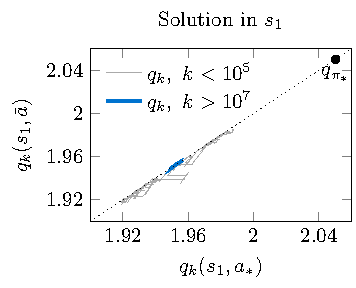
\includegraphics{figures/fv-simulation.pdf}
    % \begin{tikzpicture}
    %     \begin{axis}[
    %         width=0.9\linewidth,
    %         height=4.5cm,
    %         title={Solution in $s_1$},
    %         xmin=1.9, xmax=2.06,
    %         ymin=1.9, ymax=2.06,
    %         xlabel={$q_k(s_1,a_*)$},
    %         ylabel={$q_k(s_1,\bar a)$},
    %         xtick={1.92,1.96,2.00,2.04},
    %         ytick={1.92,1.96,2.00,2.04},
    %         legend style={
    %             draw=none,
    %             fill=none,
    %             at={(0.03,0.97)},
    %             anchor=north west
    %         },
    %         legend cell align={left},
    %         tick align=inside,
    %     ]
        
    %     % Early trajectory: q_k, k < 10^5
    %     \addplot+[
    %         mygrey,
    %         thin,
    %         mark=none
    %     ] table[
    %         x=q_star_action,
    %         y=q_bar_action,
    %         col sep=comma
    %     ] {figures/cycleplot_csv/q_early.csv};
    %     \addlegendentry{$q_k,\ k<10^5$}

    %     % \addplot+[
    %     %     blue,
    %     %     thin,
    %     %     mark=none
    %     % ] table[
    %     %     x=q_star_action,
    %     %     y=q_bar_action,
    %     %     col sep=comma
    %     % ] {figures/cycleplot_csv/q_early_late.csv};
    %     % \addlegendentry{{$q_k,\ k<10^5$}}
        
    %     % Boundary q_k(s,a_*) = q_k(s,\bar a)
    %     % \addplot+[
    %     %     red!60,
    %     %     dotted,
    %     %     thin,
    %     %     mark=none
    %     % ] table[
    %     %     x=q_star_action,
    %     %     y=q_bar_action,
    %     %     col sep=comma
    %     % ] {cycleplot_csv/boundary.csv};
    %     % \addlegendentry{boundary}
        
    %     % Optimal-policy value q_{\pi_*}
    %     % \addplot+[
    %     %     orange,
    %     %     only marks,
    %     %     mark=+,
    %     %     mark size=3pt,
    %     %     thick
    %     % ] table[
    %     %     x=q_star_action,
    %     %     y=q_bar_action,
    %     %     col sep=comma
    %     % ] {cycleplot_csv/q_pi_star.csv};
    %     % \addlegendentry{{$q_{\pi_*}$}}
        
    %     % Late trajectory: q_k, k > 10^7
    %     \addplot+[
    %         CambridgeCoreBlue,
    %         very thick,
    %         mark=none
    %     ] table[
    %         x=q_star_action,
    %         y=q_bar_action,
    %         col sep=comma
    %     ] {figures/cycleplot_csv/q_late.csv};
    %     \addlegendentry{{$q_k,\ k>10^7$}}

    %     \addplot[forget plot, dotted, black, domain=1.9:2.1, samples=2] {x};

    %     \addplot+[
    %         only marks,
    %         mark options={draw=black, fill=black},
    %         mark=*,
    %         mark size=2pt,
    %         % thick
    %     ] coordinates {(2.0504,2.0504)};
    %     \node[
    %         anchor=north
    %     ] at (axis cs:2.0504,2.0504) {$q_{\pi_*}$};
    %     \end{axis}
    %     \end{tikzpicture}
    \label{fig:cyclefig}
    \end{subfigure}
\hfill
\begin{subfigure}[b]{0.48\textwidth}
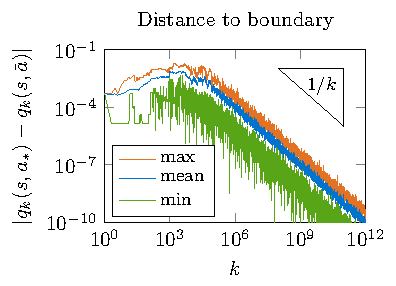
\includegraphics{figures/fv-contraction.pdf}
    % \begin{tikzpicture}
    %     \begin{axis}[
    %         width=0.9\linewidth,
    %         % height=.8\linewidth,
    %         % width=6cm,
    %         height=4.5cm,
    %         title={Distance to boundary},
    %         xmode=log,
    %         ymode=log,
    %         xmin=1,
    %         xmax=1e12,
    %         ymin=1e-10,
    %         ymax=1e-1,
    %         xtick ={1,10^(3),10^(6),10^(9),10^(12)},
    %         ytick distance=10^(3),
    %         xlabel={$k$},
    %         ylabel={$|q_k(s,a_*) - q_k(s,\bar a)|$},
    %         legend style={
    %             at={(0.03,0.03)},
    %             anchor=south west,
    %             draw=black,
    %             fill=white,
    %             font=\small
    %         },
    %         legend cell align={left},
    %         tick align=inside,
    %     ]
        
    %     \addplot+[
    %         CambridgeCoreOrange,
    %         thin,
    %         mark=none
    %     ] table[
    %         x=k,
    %         y=max_gap,
    %         col sep=comma
    %     ] {figures/cycleplot_csv/gap_stats.csv};
    %     \addlegendentry{max}

    %     \addplot+[
    %         CambridgeCoreBlue,
    %         thin,
    %         mark=none
    %     ] table[
    %         x=k,
    %         y=mean_gap,
    %         col sep=comma
    %     ] {figures/cycleplot_csv/gap_stats.csv};
    %     \addlegendentry{mean}
        
    %     \addplot+[
    %         CambridgeCoreGreen,
    %         thin,
    %         mark=none
    %     ] table[
    %         x=k,
    %         y=min_gap,
    %         col sep=comma
    %     ] {figures/cycleplot_csv/gap_stats.csv};
    %     \addlegendentry{min}
        
    %     % \addplot+[
    %     %     purple,
    %     %     thin,
    %     %     mark=none
    %     % ] table[
    %     %     x=k,
    %     %     y=ref_line,
    %     %     col sep=comma
    %     % ] {figures/cycleplot_csv/gap_stats.csv};
    %     % \addlegendentry{$0.1/k$}

    %     \draw[black] (axis cs:1e8, 1e-2) -- (axis cs:1e11, 1e-2) -- (axis cs:1e11,1e-5) -- cycle;
    %     \node[below left, font=\small] at (axis cs:1e11, 1e-2) {$1/k$};
    %     \end{axis}
    %     \end{tikzpicture}
\end{subfigure}
%     \hfill
% \begin{subfigure}[b]{0.48\textwidth}
%     \includegraphics[width=\textwidth]{gapfig}
%     \caption{gaps: $q_k(s,a_*)-q_k(s,\bar a)$}
%     \label{fig:gapfig}
% \end{subfigure}
\caption{First-visit MCES with sample-average updates can converge to a suboptimal solution where $q(s, a_*) = q(s, \bar a)$ for all states.}
\label{fig:fvsasim}
\end{figure}